\chapter{Optimizing SNSPD HBT and TCSPC measurement of a fs laser source}


\section{Motivations and experimental setup overview}
\begin{figure}[hbtp]
\centering
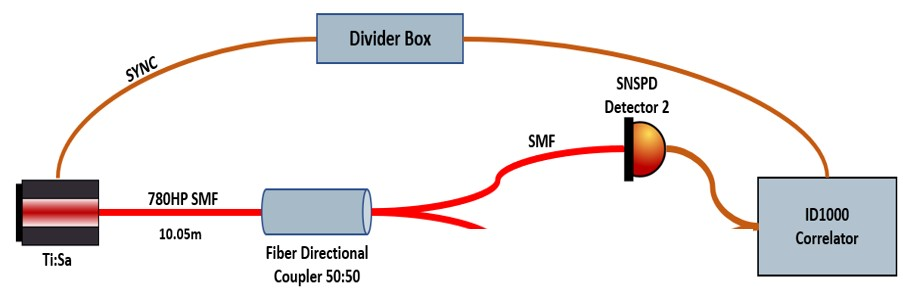
\includegraphics[width=1\textwidth]{TiSa_Setup.jpg}
\caption{Ciaone}
\label{TisaSetup}
\end{figure}



\section{Unwanted Side Peaks in HBT and TCSPC measurements}

\begin{figure}[hbtp]
\centering
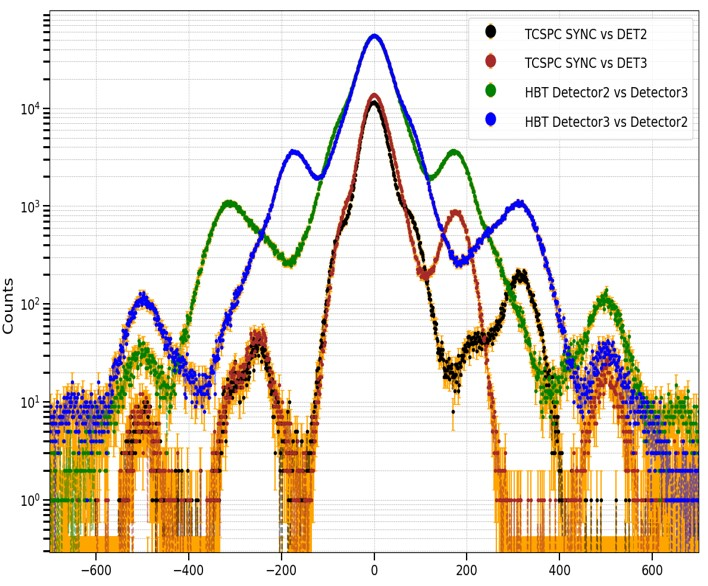
\includegraphics[width=1\textwidth]{Khaos.jpg}
\caption{Ciaone}
\label{Khaos}
\end{figure}
\section{Partly retrieving side peaks in HBT from coordinates of TCSPC peaks}

\begin{figure}[hbtp]
\centering
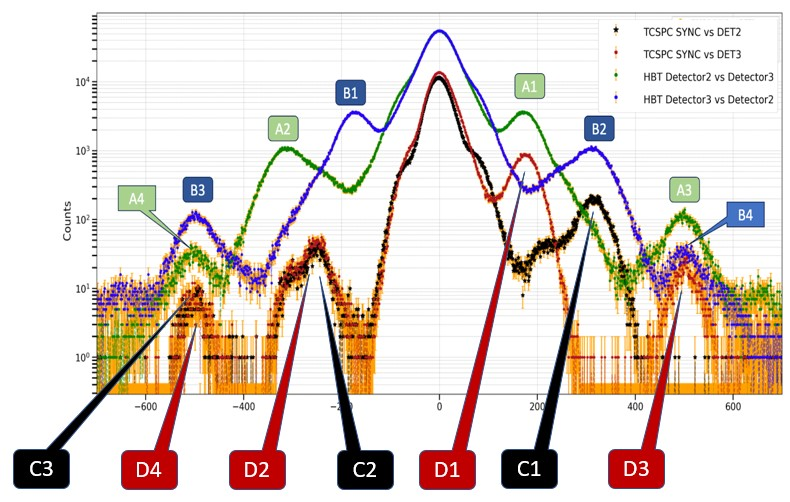
\includegraphics[width=1\textwidth]{Khaos_Labeled.jpg}
\caption{Ciaone}
\label{Khaos_labeled}
\end{figure}


\begin{table}[h!]
\centering
\caption*{\textbf{Detected position of the peaks}}
\renewcommand{\arraystretch}{1.3}
\begin{tabular}{
>{\centering\arraybackslash}m{1.5cm} 
>{\centering\arraybackslash}m{1.5cm} 
>{\centering\arraybackslash}m{1.5cm} 
>{\centering\arraybackslash}m{1.5cm} 
>{\centering\arraybackslash}m{1.5cm}}
\rowcolor{blue!50}
\textcolor{white}{\small[\textbf{ps}]} & \textcolor{white}{\textbf{A}} & \textcolor{white}{\textbf{B}} & \textcolor{white}{\textbf{C}} & \textcolor{white}{\textbf{D}} \\
\rowcolor{white}
\cellcolor{blue!50} \textcolor{white}{\textbf{0}} & 0    & 0    & 0     & 0     \\
\rowcolor{white}
\cellcolor{blue!50} \textcolor{white}{\textbf{1}} & 174  & -174 & 316   & 175   \\
\rowcolor{white}
\cellcolor{blue!50} \textcolor{white}{\textbf{2}} & -313 & 312  & -250  & -246  \\
\rowcolor{white}
\cellcolor{blue!50} \textcolor{white}{\textbf{3}} & 495  & -494 & -500  & +501  \\
\rowcolor{white}
\cellcolor{blue!50} \textcolor{white}{\textbf{4}} & -502 & 503  & n.d.  & -500  \\
\rowcolor{white}
\end{tabular}
\end{table}









\section{Measurements with improved detection thresholds}
\subsection{Driving idea}
we strongly suspect that the chaotic behavior that we're getting, although we're visualizing the data always in log scale finds its origin in a sort of miscalibration of the triggering thresholds.
For this reason we managed to shut the laser and while the detector was receiving only stray photons, we looked at the electronic pulses coming out of the SNSPD.
Subsequently we initialized the Oscilloscope to visualize also the first derivative of the pulse so that we could get an info on where to locate the new, and refined threshold. The whole idea was to choose the point where the electrical signal expressed the greatest steepness, in order to achieve better measurements.
The whole idea we formulated explained the side peaks, as a consequence of having the detector measuring clicks when it was not fully recovered from the previous detection. By Modifying for a stronger threshold, as seen in \autoref{TrickShot}, we are getting rid of the even slow possibility to trigger with a non fully recovered nanowire.
Important mention is related to how we looked at these signals : instead of plugging the cable from the SNSPD straight into the Oscilloscope, we managed to add an impedence load to it, valued $50 \Omega$, to simulate the impedence that it will encounter at the entrance of the ID1000 Time-Tagger.

\begin{figure}[hbtp]
\centering
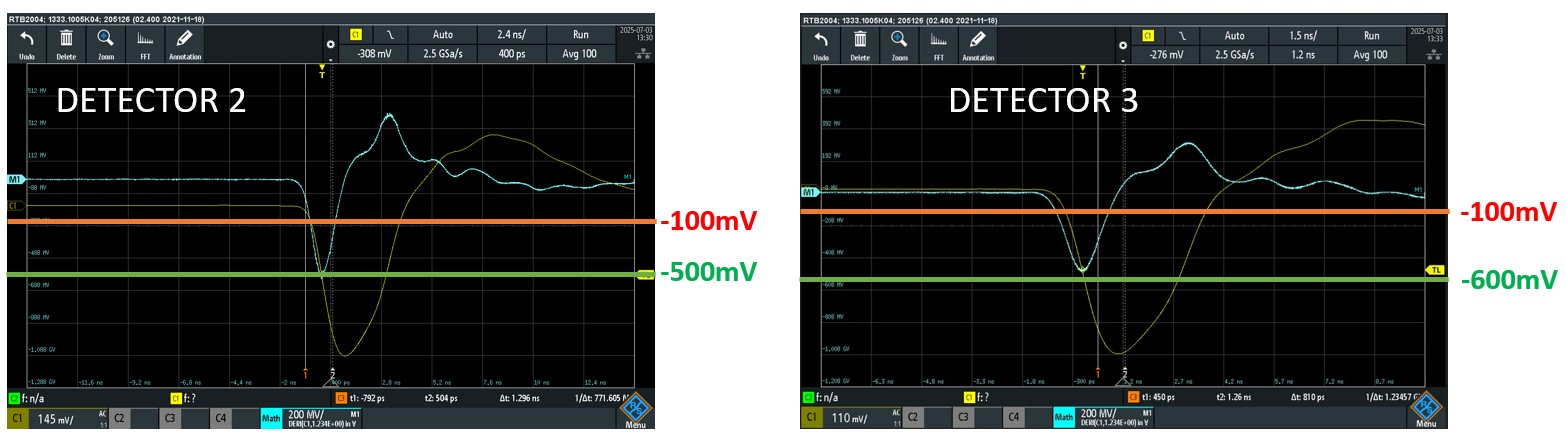
\includegraphics[width=1\textwidth]{ScopeShots.jpg}
\caption{Ciaone}
\label{TrickShot}
\end{figure}

As seen in \autoref{TrickShot}, by looking at the images we significantly modified the thresholds, passing from a value of $-100mV$ for both the detectors to $-500mV$ and $-600mV$, for detector 2 and detector 3 respectively.

\subsection{Discussion of the new measurements}
\begin{figure}[hbtp]
\centering
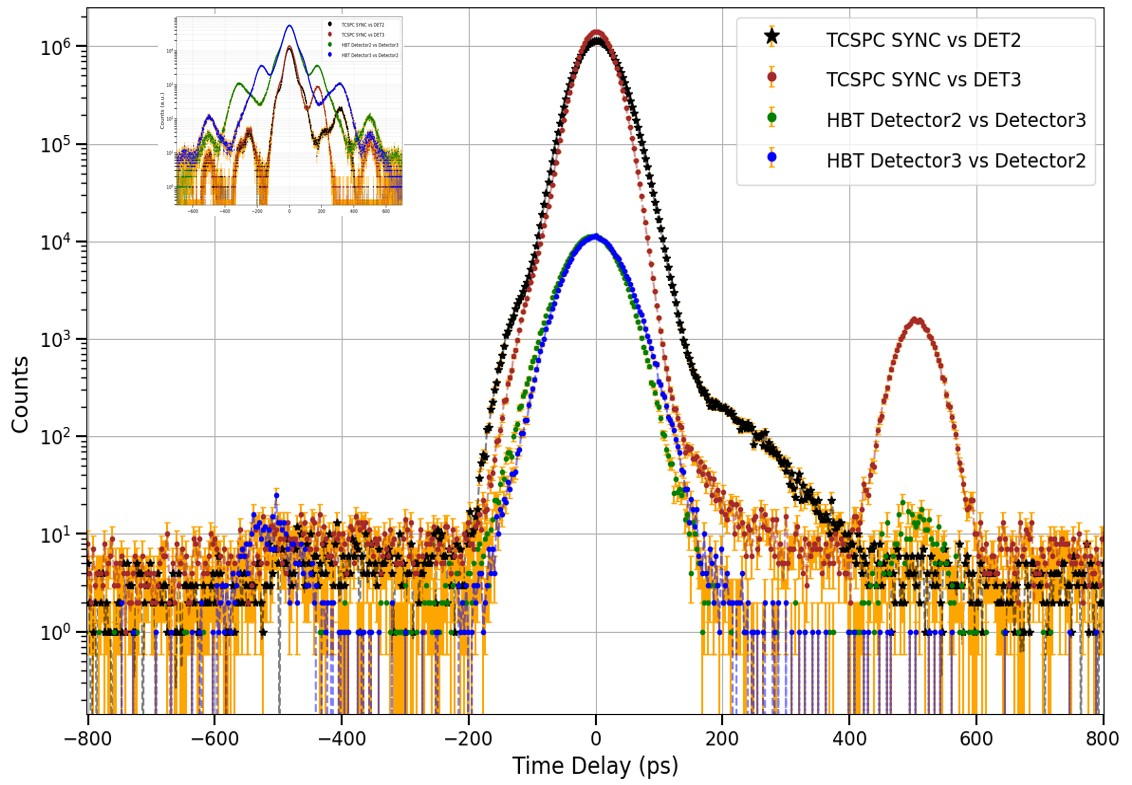
\includegraphics[width=1\textwidth]{CheckpointBravo_vs_Khaos.jpg}
\caption{Ciaone}
\label{RefinedMeasurement}
\end{figure}


% \subsection{Estimation of the width of the Detector response function}